%%%%%%%%%%%%  Generated using docx2latex.com  %%%%%%%%%%%%%%

%%%%%%%%%%%%  v2.0.0-beta  %%%%%%%%%%%%%%

\documentclass[12pt]{article}
\usepackage{amsmath}
\usepackage{latexsym}
\usepackage{amsfonts}
\usepackage[normalem]{ulem}
\usepackage{array}
\usepackage{amssymb}
\usepackage{graphicx}
\usepackage[backend=biber,
style=numeric,
sorting=none,
isbn=false,
doi=false,
url=false,
]{biblatex}\addbibresource{bibliography.bib}

\usepackage{subfig}
\usepackage{wrapfig}
\usepackage{wasysym}
\usepackage{enumitem}
\usepackage{adjustbox}
\usepackage{ragged2e}
\usepackage[svgnames,table]{xcolor}
\usepackage{tikz}
\usepackage{longtable}
\usepackage{changepage}
\usepackage{setspace}
\usepackage{hhline}
\usepackage{multicol}
\usepackage{tabto}
\usepackage{float}
\usepackage{multirow}
\usepackage{makecell}
\usepackage{fancyhdr}
\usepackage[toc,page]{appendix}
\usepackage[hidelinks]{hyperref}
\usetikzlibrary{shapes.symbols,shapes.geometric,shadows,arrows.meta}
\tikzset{>={Latex[width=1.5mm,length=2mm]}}
\usepackage{flowchart}\usepackage[paperheight=11.0in,paperwidth=8.5in,left=1.0in,right=1.0in,top=1.0in,bottom=1.0in,headheight=1in]{geometry}
\usepackage[utf8]{inputenc}
\usepackage[T1]{fontenc}
\TabPositions{0.5in,1.0in,1.5in,2.0in,2.5in,3.0in,3.5in,4.0in,4.5in,5.0in,5.5in,6.0in,}

\urlstyle{same}


 %%%%%%%%%%%%  Set Depths for Sections  %%%%%%%%%%%%%%

% 1) Section
% 1.1) SubSection
% 1.1.1) SubSubSection
% 1.1.1.1) Paragraph
% 1.1.1.1.1) Subparagraph


\setcounter{tocdepth}{5}
\setcounter{secnumdepth}{5}


 %%%%%%%%%%%%  Set Depths for Nested Lists created by \begin{enumerate}  %%%%%%%%%%%%%%


\setlistdepth{9}
\renewlist{enumerate}{enumerate}{9}
		\setlist[enumerate,1]{label=\arabic*)}
		\setlist[enumerate,2]{label=\alph*)}
		\setlist[enumerate,3]{label=(\roman*)}
		\setlist[enumerate,4]{label=(\arabic*)}
		\setlist[enumerate,5]{label=(\Alph*)}
		\setlist[enumerate,6]{label=(\Roman*)}
		\setlist[enumerate,7]{label=\arabic*}
		\setlist[enumerate,8]{label=\alph*}
		\setlist[enumerate,9]{label=\roman*}

\renewlist{itemize}{itemize}{9}
		\setlist[itemize]{label=$\cdot$}
		\setlist[itemize,1]{label=\textbullet}
		\setlist[itemize,2]{label=$\circ$}
		\setlist[itemize,3]{label=$\ast$}
		\setlist[itemize,4]{label=$\dagger$}
		\setlist[itemize,5]{label=$\triangleright$}
		\setlist[itemize,6]{label=$\bigstar$}
		\setlist[itemize,7]{label=$\blacklozenge$}
		\setlist[itemize,8]{label=$\prime$}

\setlength{\topsep}{0pt}\setlength{\parindent}{0pt}

 %%%%%%%%%%%%  This sets linespacing (verticle gap between Lines) Default=1 %%%%%%%%%%%%%%


\renewcommand{\arraystretch}{1.3}


%%%%%%%%%%%%%%%%%%%% Document code starts here %%%%%%%%%%%%%%%%%%%%



\begin{document}
\begin{Center}
\textbf{\textit{Assignment 2}}
\end{Center}\par


\vspace{\baselineskip}
\begin{Center}
\textbf{\textit{Prashant Lawhatre (17510056)}}
\end{Center}\par


\vspace{\baselineskip}
\begin{Center}
\textbf{\textit{September 9, 2018}}
\end{Center}\par


\vspace{\baselineskip}

\vspace{\baselineskip}
\uline{Answer to Question 2}\par


\vspace{\baselineskip}
\begin{enumerate}
	\item [J,T]=histeq(I)
\end{enumerate}\par

\begin{enumerate}
	\item 1.jpg
\end{enumerate}\par



%%%%%%%%%%%%%%%%%%%% Figure/Image No: 1 starts here %%%%%%%%%%%%%%%%%%%%

\begin{figure}[H]
	\begin{Center}
		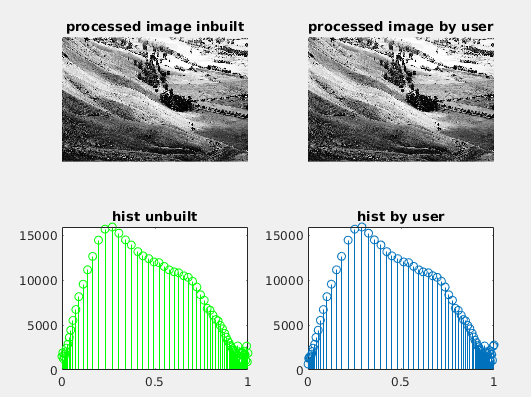
\includegraphics[width=3.82in,height=2.85in]{./media/image8.png}
	\end{Center}
\end{figure}


%%%%%%%%%%%%%%%%%%%% Figure/Image No: 1 Ends here %%%%%%%%%%%%%%%%%%%%

\par

\begin{adjustwidth}{1.0in}{0.0in}
\begin{Center}
Fig 1-Processed image by inbuilt and user-defined function with histograms
\end{Center}\par

\end{adjustwidth}


\vspace{\baselineskip}


%%%%%%%%%%%%%%%%%%%% Figure/Image No: 2 starts here %%%%%%%%%%%%%%%%%%%%

\begin{figure}[H]
	\begin{Center}
		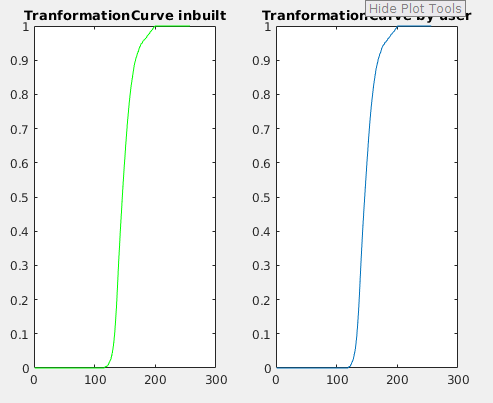
\includegraphics[width=3.96in,height=2.77in]{./media/image15.png}
	\end{Center}
\end{figure}


%%%%%%%%%%%%%%%%%%%% Figure/Image No: 2 Ends here %%%%%%%%%%%%%%%%%%%%

\begin{adjustwidth}{1.0in}{0.0in}
\begin{Center}
 
\end{Center}\par

\end{adjustwidth}

\begin{adjustwidth}{1.0in}{0.0in}
\begin{Center}
Fig 2- T vector curves obtained by inbuilt and user defined function
\end{Center}\par

\end{adjustwidth}


\vspace{\baselineskip}
\begin{adjustwidth}{1.0in}{0.0in}
\begin{justify}
\textit{Comments:}From fig 1 we can say that both the processed images obtained after applying inbuilt and user defined function are sam.Also, the histograms are same. Similarly, from fig 2 Transformation vectors are also same.
\end{justify}\par

\end{adjustwidth}


\vspace{\baselineskip}
\begin{justify}
\tab b) cameraman.tif
\end{justify}\par


\vspace{\baselineskip}


%%%%%%%%%%%%%%%%%%%% Figure/Image No: 3 starts here %%%%%%%%%%%%%%%%%%%%

\begin{figure}[H]
	\begin{Center}
		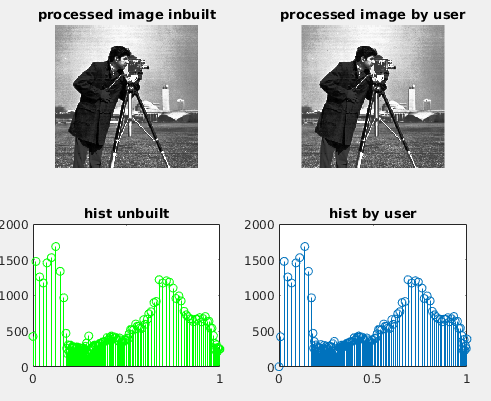
\includegraphics[width=3.57in,height=2.91in]{./media/image17.png}
	\end{Center}
\end{figure}


%%%%%%%%%%%%%%%%%%%% Figure/Image No: 3 Ends here %%%%%%%%%%%%%%%%%%%%

\tab \tab \par

\begin{adjustwidth}{1.0in}{0.0in}
\begin{Center}
Fig 3-Processed image by inbuilt and user-defined function with histograms
\end{Center}\par

\end{adjustwidth}


\vspace{\baselineskip}


%%%%%%%%%%%%%%%%%%%% Figure/Image No: 4 starts here %%%%%%%%%%%%%%%%%%%%

\begin{figure}[H]
	\begin{Center}
		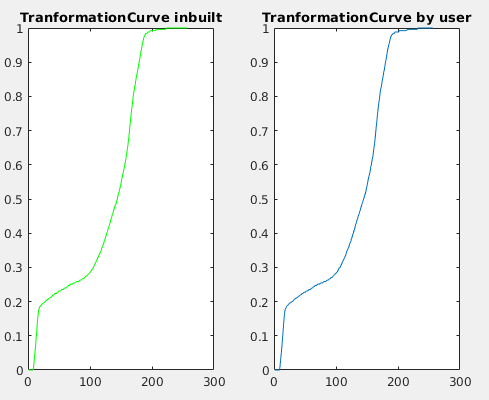
\includegraphics[width=3.75in,height=2.5in]{./media/image22.png}
	\end{Center}
\end{figure}


%%%%%%%%%%%%%%%%%%%% Figure/Image No: 4 Ends here %%%%%%%%%%%%%%%%%%%%

\begin{Center}
\ \ \ \ \ \ \ \ \ \ \ \ \ \ \ \ \ \ \ \ \ \ \ \ \ \ \ \ \ \  
\end{Center}\par

\begin{adjustwidth}{1.0in}{0.0in}
\begin{Center}
Fig 4- T vector curves obtained by inbuilt and user defined function
\end{Center}\par

\end{adjustwidth}


\vspace{\baselineskip}
\begin{adjustwidth}{1.0in}{0.0in}
\begin{justify}
\textit{Comments:}From fig 3 we can say that both the processed images obtained after applying inbuilt and user defined function are sam.Also, the histograms are same. Similarly, from fig 4 Transformation vectors are also same.
\end{justify}\par

\end{adjustwidth}


\vspace{\baselineskip}
\begin{justify}
2) J=histeq(I,n)
\end{justify}\par

\begin{enumerate}
	\item 1.jpg
\end{enumerate}\par



%%%%%%%%%%%%%%%%%%%% Figure/Image No: 5 starts here %%%%%%%%%%%%%%%%%%%%

\begin{figure}[H]
	\begin{Center}
		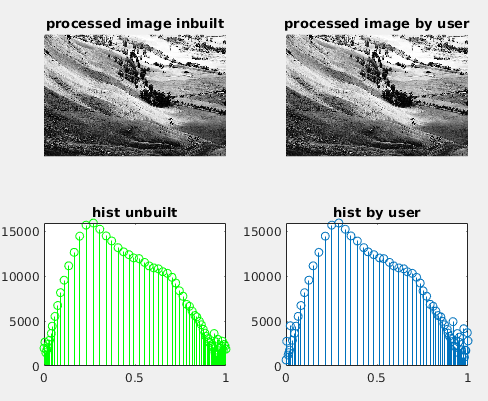
\includegraphics[width=3.38in,height=2.78in]{./media/image21.png}
	\end{Center}
\end{figure}


%%%%%%%%%%%%%%%%%%%% Figure/Image No: 5 Ends here %%%%%%%%%%%%%%%%%%%%

\par

\begin{adjustwidth}{1.0in}{0.0in}
\begin{Center}
Fig 5-Processed image by inbuilt and user-defined function with histograms with 200 bins
\end{Center}\par

\end{adjustwidth}


\vspace{\baselineskip}
\begin{adjustwidth}{1.0in}{0.0in}
\begin{justify}
\textit{Comments:}From fig 5 we can say that both the processed images obtained after applying inbuilt and user defined function are same for number of bins provided.
\end{justify}\par

\end{adjustwidth}


\vspace{\baselineskip}
\begin{justify}
\tab b) pout.tif\tab \tab 
\end{justify}\par


\vspace{\baselineskip}


%%%%%%%%%%%%%%%%%%%% Figure/Image No: 6 starts here %%%%%%%%%%%%%%%%%%%%

\begin{figure}[H]
	\begin{Center}
		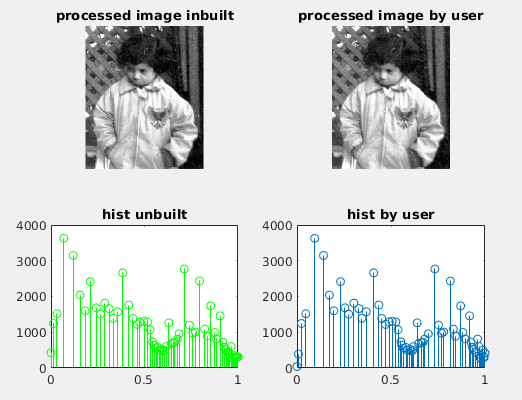
\includegraphics[width=3.41in,height=2.61in]{./media/image7.png}
	\end{Center}
\end{figure}


%%%%%%%%%%%%%%%%%%%% Figure/Image No: 6 Ends here %%%%%%%%%%%%%%%%%%%%

\par

\begin{adjustwidth}{1.0in}{0.0in}
\begin{Center}
Fig 6-Processed image by inbuilt and user-defined function with histograms with 220 bins
\end{Center}\par

\end{adjustwidth}


\vspace{\baselineskip}
\begin{adjustwidth}{1.0in}{0.0in}
\begin{justify}
\textit{Comments:}From fig 6 we can say that both the processed images obtained after applying inbuilt and user defined function are same for number of bins provided.
\end{justify}\par

\end{adjustwidth}


\vspace{\baselineskip}

\vspace{\baselineskip}
\tab 
\vspace{\baselineskip}\begin{justify}
\tab c) cameraman.tif
\end{justify}\par


\vspace{\baselineskip}


%%%%%%%%%%%%%%%%%%%% Figure/Image No: 7 starts here %%%%%%%%%%%%%%%%%%%%

\begin{figure}[H]
	\begin{Center}
		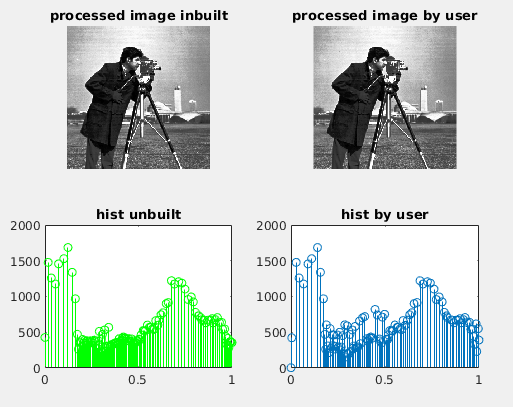
\includegraphics[width=4.08in,height=3.24in]{./media/image16.png}
	\end{Center}
\end{figure}


%%%%%%%%%%%%%%%%%%%% Figure/Image No: 7 Ends here %%%%%%%%%%%%%%%%%%%%

\tab \tab \par

\begin{adjustwidth}{1.0in}{0.0in}
\begin{Center}
Fig 7-Processed image by inbuilt and user-defined function with histograms with 180 bins
\end{Center}\par

\end{adjustwidth}

\begin{adjustwidth}{1.0in}{0.0in}
\begin{justify}
\textit{Comments:}From fig 7 we can say that both the processed images obtained after applying inbuilt and user defined function are same for number of bins provided.
\end{justify}\par

\end{adjustwidth}


\vspace{\baselineskip}
\begin{justify}
3) J=histeq(I,I1,verbose\_fig)
\end{justify}\par

\begin{enumerate}
	\item Source image histogram= pout.tif, target image histogram=cameraman.tif
\end{enumerate}\par

\tab 
\vspace{\baselineskip}

%%%%%%%%%%%%%%%%%%%% Figure/Image No: 8 starts here %%%%%%%%%%%%%%%%%%%%

\begin{figure}[H]
	\begin{Center}
		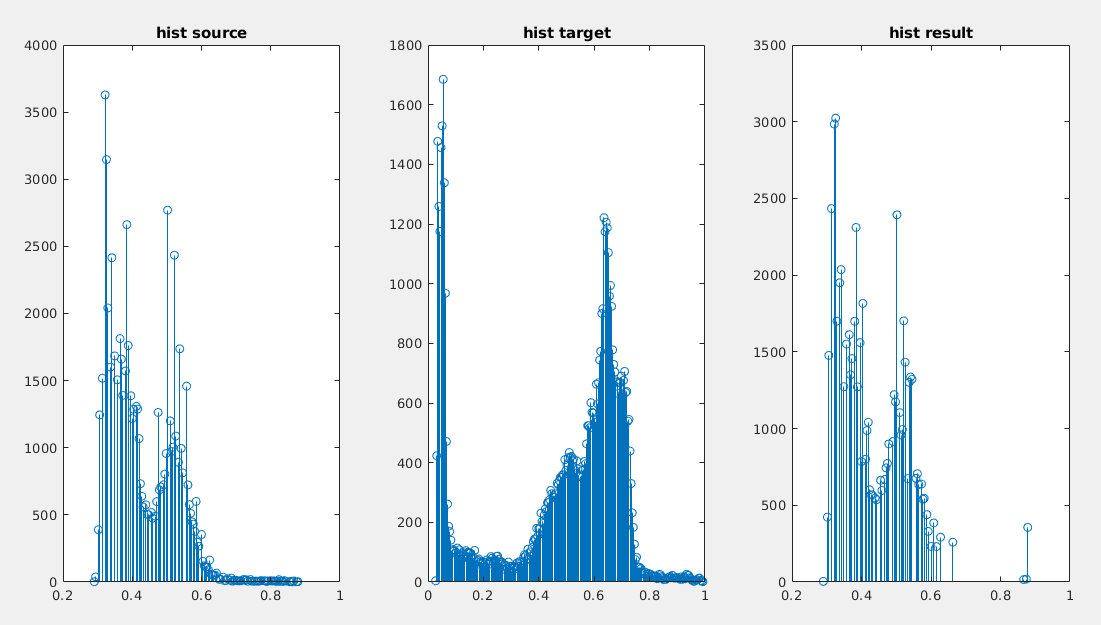
\includegraphics[width=4.51in,height=2.56in]{./media/image19.png}
	\end{Center}
\end{figure}


%%%%%%%%%%%%%%%%%%%% Figure/Image No: 8 Ends here %%%%%%%%%%%%%%%%%%%%

\par

\begin{Center}
Fig 8- Histograms of the source image, target image and the resultant image
\end{Center}\par


\vspace{\baselineskip}
\begin{adjustwidth}{1.0in}{0.0in}
\begin{justify}
\textit{Comments:}From fig., we can say that the source image has roughly matched to the target image.
\end{justify}\par

\end{adjustwidth}

\begin{justify}
\ \  b) Source image histogram= cameraman.tif, target image histogram=1.jpg
\end{justify}\par

\tab \tab 
\vspace{\baselineskip}

%%%%%%%%%%%%%%%%%%%% Figure/Image No: 9 starts here %%%%%%%%%%%%%%%%%%%%

\begin{figure}[H]
	\begin{Center}
		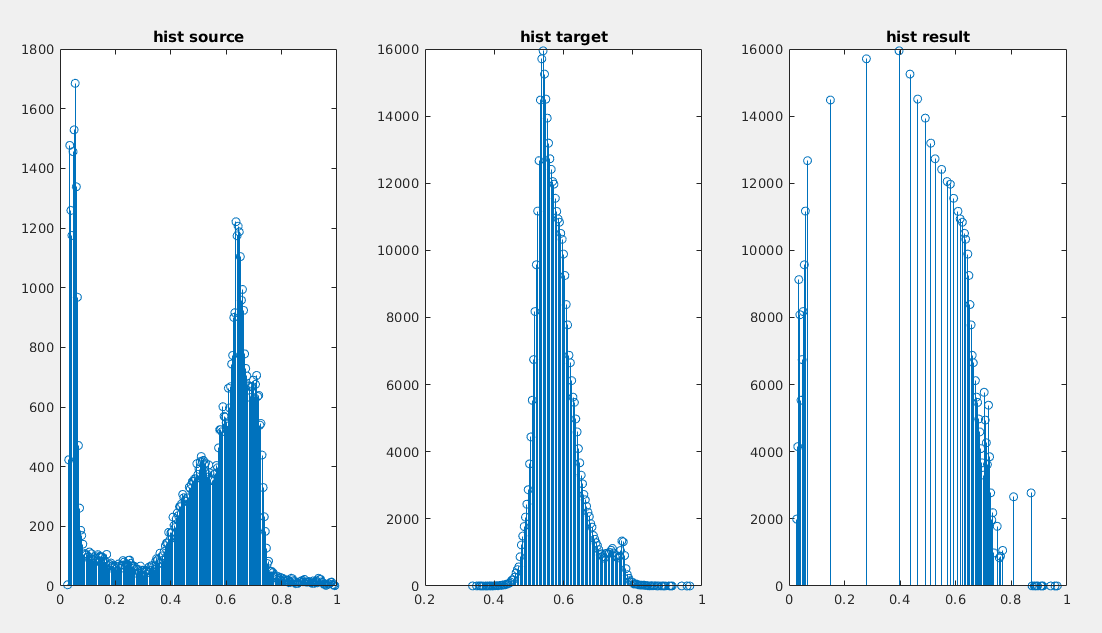
\includegraphics[width=3.93in,height=2.26in]{./media/image18.png}
	\end{Center}
\end{figure}


%%%%%%%%%%%%%%%%%%%% Figure/Image No: 9 Ends here %%%%%%%%%%%%%%%%%%%%

\par

\begin{Center}
Fig 9- Histograms of the source image, target image and the resultant image
\end{Center}\par


\vspace{\baselineskip}
\begin{adjustwidth}{1.0in}{0.0in}
\begin{justify}
\textit{Comments:}From fig., we can say that the source image has roughly matched to the target image.
\end{justify}\par

\end{adjustwidth}


\vspace{\baselineskip}
\begin{justify}
\  c) Source image histogram= pout.tif, target image histogram=1.jpg
\end{justify}\par



%%%%%%%%%%%%%%%%%%%% Figure/Image No: 10 starts here %%%%%%%%%%%%%%%%%%%%

\begin{figure}[H]
	\begin{Center}
		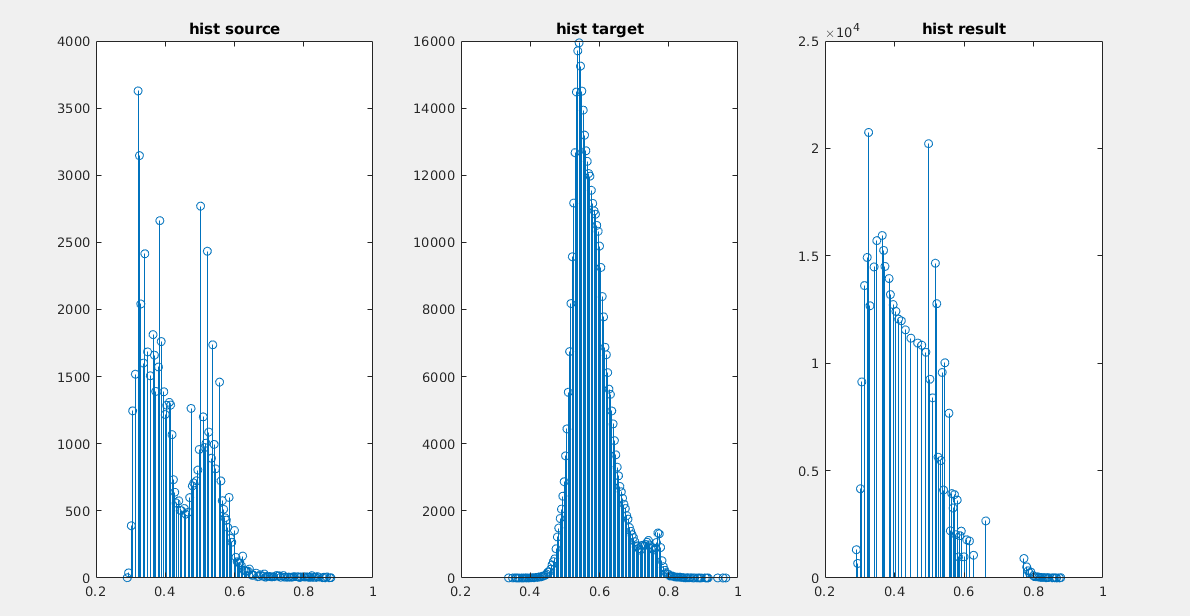
\includegraphics[width=4.32in,height=2.23in]{./media/image14.png}
	\end{Center}
\end{figure}


%%%%%%%%%%%%%%%%%%%% Figure/Image No: 10 Ends here %%%%%%%%%%%%%%%%%%%%

\par

\begin{Center}
Fig 10- Histograms of the source image, target image and the resultant image
\end{Center}\par


\vspace{\baselineskip}
\begin{adjustwidth}{1.0in}{0.0in}
\begin{justify}
\textit{Comments:}From fig., we can say that the source image has roughly matched to the target image.
\end{justify}\par

\end{adjustwidth}


\vspace{\baselineskip}

\vspace{\baselineskip}

\vspace{\baselineskip}

\vspace{\baselineskip}

\vspace{\baselineskip}

\vspace{\baselineskip}

\vspace{\baselineskip}

\vspace{\baselineskip}
\begin{justify}
4) J=histeq(I,hgram)
\end{justify}\par

\begin{justify}
\tab a)cameraman.tif 
\end{justify}\par



%%%%%%%%%%%%%%%%%%%% Figure/Image No: 11 starts here %%%%%%%%%%%%%%%%%%%%

\begin{figure}[H]
	\begin{Center}
		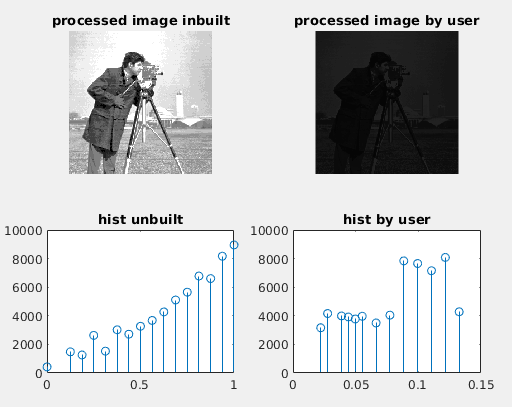
\includegraphics[width=3.06in,height=2.43in]{./media/image20.png}
	\end{Center}
\end{figure}


%%%%%%%%%%%%%%%%%%%% Figure/Image No: 11 Ends here %%%%%%%%%%%%%%%%%%%%

\begin{Center}
\ \ \ \ \ \ \ \ \ \ \ \ \ \ \ \ \ \ \ \ \ \ \  \tab 
\end{Center}\par

\begin{adjustwidth}{1.0in}{0.0in}
\begin{Center}
Fig 11- Processed image and their histograms by inbuilt and 
\end{Center}\par

\end{adjustwidth}

\begin{Center}
\ \ \ \ \ \ \ \ \ \ \ \ \ \ \ \ \ \ \ \ \ \ \ \ \ \ \ \ \ \ \ \ \ \ \ \ \  user defined functions
\end{Center}\par

\ \ \ \ \ \ \ \ \ \ \ \ \ \ \ \ \ \ \ \ \ \ \ \ \  \textit{Comments: }The histograms of both the images is very slightly matching.\par

\tab \tab 
\vspace{\baselineskip}\begin{justify}
\tab b) 1.jpg
\end{justify}\par



%%%%%%%%%%%%%%%%%%%% Figure/Image No: 12 starts here %%%%%%%%%%%%%%%%%%%%

\begin{figure}[H]
	\begin{Center}
		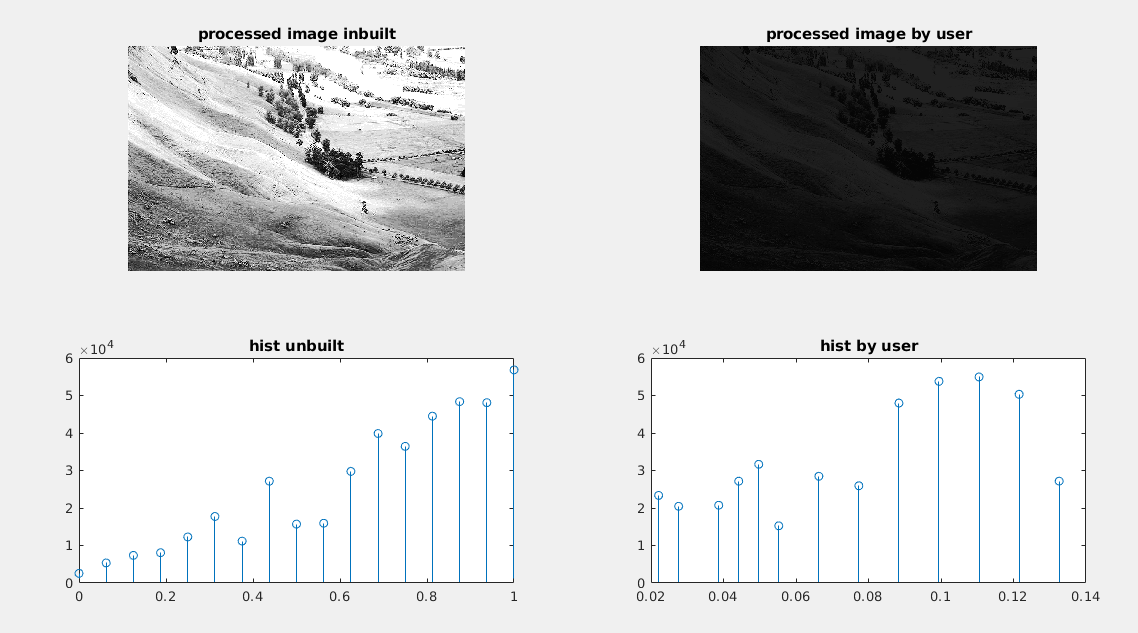
\includegraphics[width=3.5in,height=2.61in]{./media/image24.png}
	\end{Center}
\end{figure}


%%%%%%%%%%%%%%%%%%%% Figure/Image No: 12 Ends here %%%%%%%%%%%%%%%%%%%%

\tab \par

\begin{adjustwidth}{1.0in}{0.0in}
\begin{Center}
Fig 12- Processed image and their histograms by inbuilt and 
\end{Center}\par

\end{adjustwidth}

\begin{Center}
\ \ \ \ \ \ \ \ \ \ \ \ \ \ \ \ \ \ \ \ \ \ \ \ \ \ \ \ \ \ \ \ \ \ \ \ \  user defined functions
\end{Center}\par

\begin{FlushLeft}
\tab \tab \textit{Comments: }The histograms of both the images is very slightly matching.
\end{FlushLeft}\par


\printbibliography
\end{document}